\chapter{Testen der Ergebnisse}
\label{kap5}

todo

\section{Visualisierung}

Gazebo

Debugging

Matplotlib

\section{Laufplanung}

\subsection{Dreifußgang}

\subsection{Random Sampling}

\autoref{kap5:footCenterMovements} bla \autoref{kap5:footDown}

\begin{figure}[b!]
  \centering
  \begin{subfigure}[b]{.5\linewidth}
    \centering
    \includegraphics[scale=0.45]{kapitel5/footdownSuccess1}
    \subcaption{Direkte Suche}\label{kap5:footDownNormal2}
  \end{subfigure}%
  \begin{subfigure}[b]{.5\linewidth}
    \centering
    \includegraphics[scale=0.45]{kapitel5/footdownSuccess2}
    \subcaption{Direkte Suche}\label{kap5:footDownNormal2}
  \end{subfigure}\\
  \\[\smallskipamount]
  \begin{subfigure}[b]{.5\linewidth}
    \centering
    \includegraphics[scale=0.45]{kapitel5/footdownnoSuccess1}
    \subcaption{Spiralsuche}\label{kap5:footDownSpiral1}
  \end{subfigure}%
  \begin{subfigure}[b]{.5\linewidth}
    \centering
    \includegraphics[scale=0.45]{kapitel5/footdownnoSuccess2}
    \subcaption{Spiralsuche}\label{kap5:footDownSpiral2}
  \end{subfigure}%
  \caption{Auswertung der Positionsfindung beim Absetzen eines Fußes}
  \label{kap5:footDown}
\end{figure}

\begin{figure}[t!]
    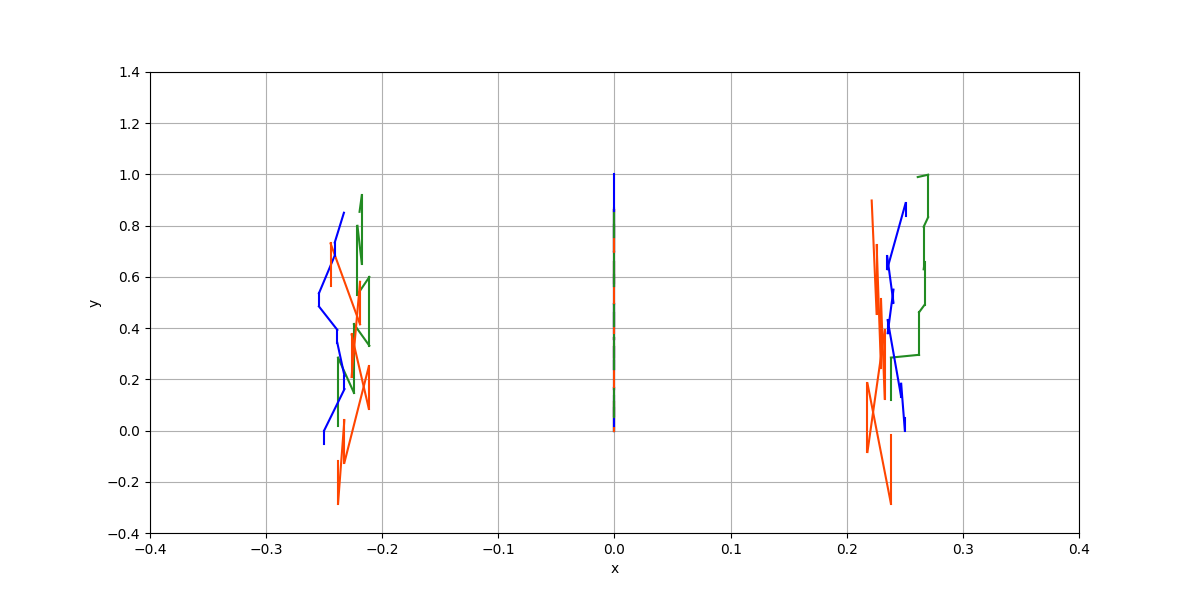
\includegraphics[width=1\textwidth]{kapitel5/footmov1}\hfill
    \\[\smallskipamount]
    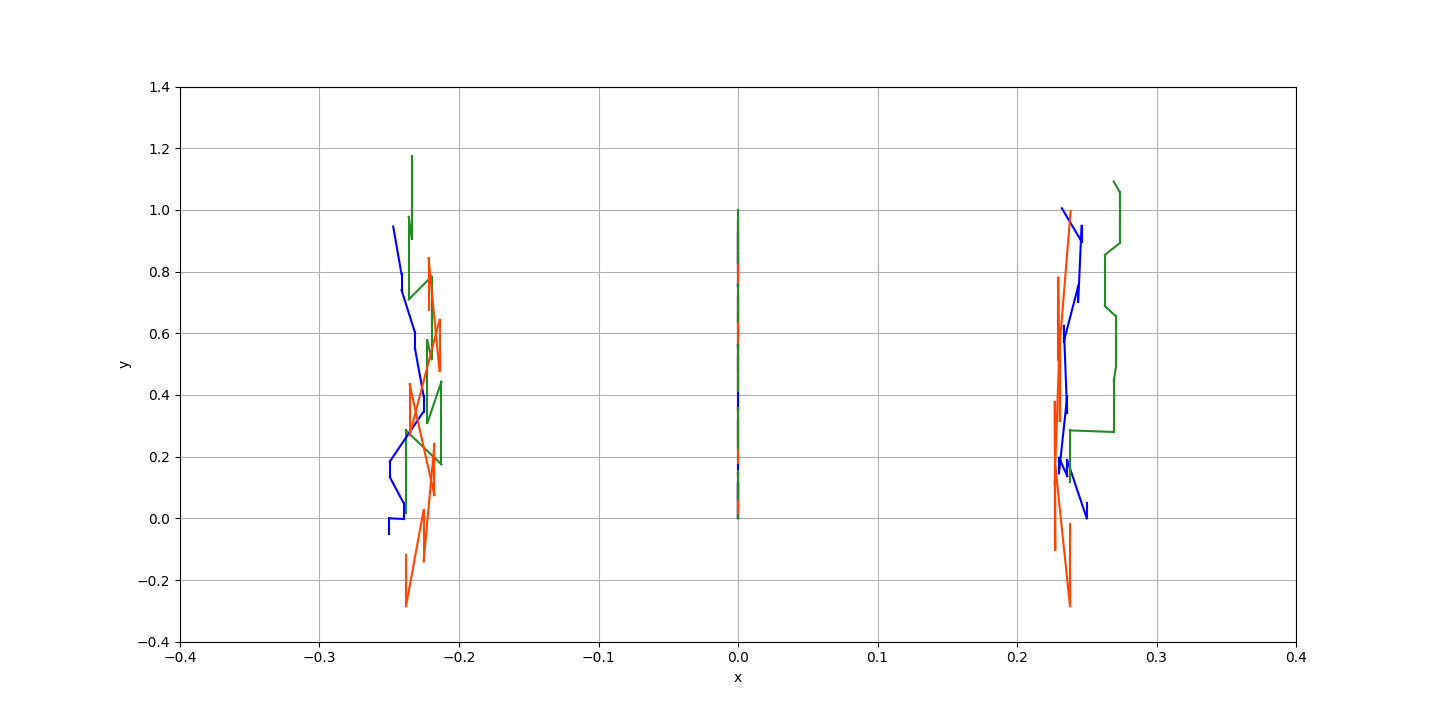
\includegraphics[width=1\textwidth]{kapitel5/footmov2}\hfill
    \\[\smallskipamount]
    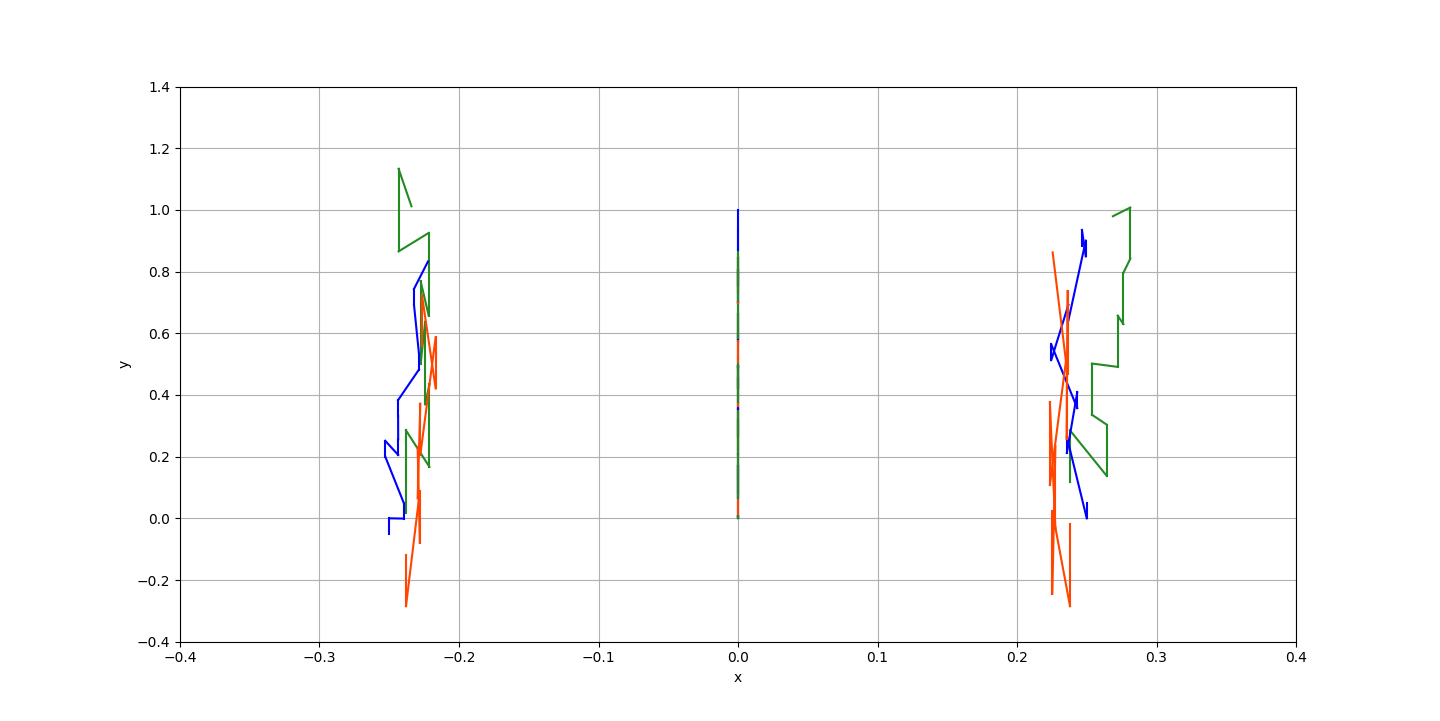
\includegraphics[width=1\textwidth]{kapitel5/footmov3}\hfill
    \caption{Auswertung von Bewegungen von Körper und Füßen}\label{kap5:footCenterMovements}
\end{figure}